\chapter{Construção da Ferramenta~\label{chp:construção-da-ferramenta}}

A ferramenta construída neste trabalho, nomeada \textit{\textbf{tjscraper}},
foi produzida para ser capaz de extrair com qualidade
satisfatória~\todofootnote{(Definir ``qualidade satisfatória'' --- em resumo:
um formato que dê de usar os dados para alguma coisa e que não seja ``grego''
para alguém que não seja da área)} os dados especificamente do TJ do Rio de
Janeiro (TJ-RJ). As estratégias empregadas, portanto, levam em conta acessos
que todos os acessos serão ao TJ-RJ, ainda que visando a possibilidade de serem
aplicadas às páginas dos TJs dos demais estados.

\section{Ferramentas utilizadas~\label{section:ferramentas-utilizadas}}

\textcolor{blue}{--->> O que estás propondo para descrição de ferramentas
(Scrapy e SQLLite) será um pequeno parágrafo de uma Seção chamada "Ferramentas
utilizadas" no capítulo de construção da ferramenta. Não vais descrever nenhuma
delas com detalhes, pois são ferramentas simplesmente usadas para contruíres
teu trabalho. Isso não se detalha porque não são "conceitos". Ferramentas mudam
de versão, saem de linha, ficam obsoletas, perdem valor, etc, portanto, não se
descrevem em detalhes.}

\todo{%
    Esta seção deve ser uma descrição das ferramentas mais relevantes que foram
    \textit{utilizadas} no trabalho, i.e. as dependências (bibliotecas,
    linguagem de programação).
}
\begin{todolist}
    \item Scrapy
    \item SQLite
    \item \ldots
\end{todolist}

\section{Organização geral}

\begin{todolist}
    \item Explicar a construção da ferramenta como CLI, biblioteca e como
          aplicação Web;
    \item Diagramar módulos;
\end{todolist}

A ferramenta foi projetada como uma biblioteca de \textit{software} acompanhada
de duas interfaces de usuário~\footnote{Neste ponto, ``usuário'' refere-se a
alguém que não esteja utilizando a ferramenta como uma biblioteca de software,
e sim como aplicação.}: uma aplicação de Interface de Linha de Comando
(\textit{ILC}\footnote{Comumente referenciado com a sigla em inglês ``CLI'', de
``Command Line Interface''.} e uma aplicação de servidor Web.

A ILC tem como objetivo permitir o uso de boa parte dos diferentes recursos da
biblioteca em um terminal para a execução tarefas pontuais, como exibir
informações sobre estado atual da \textit{cache}, iniciar um processo de
extração, ou mesmo iniciar uma instância de servidor Web da ferramenta para
fins de desenvolvimento.

O servidor Web é destinado ao usuário que queira uma interface de simples
acesso e uso da ferramenta, primariamente focando na obtenção de dados dos TJs
com os recursos que não estejam disponíveis nas páginas oficiais dos TJs
(descritos na~\todo{Referenciar Seção}), tendo em mente como público alvo
jornalistas.

\section{Estratégias de extração}

O TJ-RJ possui rotas e subdomínios que dão acesso aos mesmos dados por vias
diferentes. Delas, foram elaboradas estratégias para extrair dados da rota que
os fornece em formato HTML~\footnote{\todo{link da rota HTML}}, conhecida antes
da produção efetiva da ferramenta, e da que os fornece em formato
JSON~\footnote{\todo{link da rota JSON}}, encontrada durante o processo de
produção e portanto implementada posteriormente. O formato HTML é apresentado
como uma página de consulta para um usuário comum, enquanto o formato JSON é
um conjunto de rotas que implementam uma API Web.

A extração, em todos os casos, leva em conta a busca pelo número do processo.
Foi escolhido esse campo de busca por conta do domínio de valores válidos ser
limitado e conhecido: números de processos são dados seguindo os formatos
numéricos fixos unificado e antigo, respectivamente
``NNNNNNN-NN.AAAA.N.NN.NNNN'' e ``AAAA.NNN.NNNNNN-N'' em que ``AAAA'' é o ano
de criação do documento do processo e cada ``N'' é um dígito de 0 a 9, logo é
possível encontrar todos os processos apenas fixando o ano e testando
diferentes combinações para os demais dígitos. Outros campos, como nome das
partes por exemplo, possuem uma abrangência de valores muito grande e difícil
de se conhecer em sua totalidade ou, nos casos como a busca por Sentença, não
são capazes de, mesmo exauridas todas as combinações de valores de entrada, dar
acesso a todos os processos registrados.

\subsection{Estratégia inicial: extração HTML}

\begin{todolist}
    \item Iniciar descrevendo como um usuário comum faz uma busca por número do processo.
    \item Descrever a situação inicial das páginas do TJ-RJ;
    \item Ressaltar dificuldades com páginas diferentes, fornecendo links para
          exemplos --- para fins de reprodutibilidade, o link será uma cópia
          para um .html salvo no repositório do código da ferramenta, na pasta
          de ``samples'' (amostras);
    \item Explicar como Scrapy foi utilizado.
\end{todolist}

\review{Para extração das rotas do TJ-RJ que fornecem seu conteúdo no formato
HTML, a estratégia é semelhante a reproduzir o acesso de um usuário comum ao
efetuar uma busca. A rota de Consultas Processuais
unificada~\footnote{\url{http://www4.tjrj.jus.br/ConsultaUnificada/consulta.do}}
exibe uma página que permite a busca por processos por ambos os tipos de
numeração.}

Os resultados de consulta processual do TJ-RJ em HTML são os das requisições
feitas ao subdomínio \url{ww4.tjrj.jus.br}. A estratégia de extração dos
processos que ele disponibiliza é aproveitar que a identificação de qual
processo está sendo visualizado pode ser feita através do parâmetro de URL
\texttt{numProcesso}, cujo valor é o número do processo na numeração antiga,
efetuando requisições para a mesma URL variando apenas esse parâmetro com um
número de processo. Cada requisição pode retornar uma página de processo
válido, inexistente~\footnote{Exemplo de URL de processo inexistente:
\url{http://www4.tjrj.jus.br/consultaProcessoWebV2/consultaProc.do?numProcesso=2020.004.015548-9}},
de numeração inválida~\footnote{Exemplo de URL de processo inválido:
\url{http://www4.tjrj.jus.br/consultaProcessoWebV2/consultaMov.do?numProcesso=0}}
ou de Captcha (caso esteja fora do horário noturno~\footnote{\todo{Definir
horário noturno em alguma seção anterior.}}).

\newcommand{\urlProcValido}{\url{%
    http://www4.tjrj.jus.br/consultaProcessoWebV2/consultaProc.do?numProcesso=2021.004.015548-9
}}

Uma página de resultado da consulta pública do subdomínio ww4 do TJ-RJ para um
número de processo válido~\footnote{\urlProcValido}
(\Cref{fig:exemplo-pagina-ww4}) apresenta os campos dos dados do processo em
uma \textit{tag} HTML \texttt{<table>}, de forma que cada linha visual
corresponde a uma \textit{tag} \texttt{tr} composta por duas \textit{tags}
\texttt{td}: uma para o nome do campo e outra para o valor
(\Cref{cod:html-assunto}). Assim, um campo ``A'' pode ser encontrado procurando
por uma \texttt{td} cujo conteúdo seja ``A:'', e o valor é o próximo vizinho
considerando hierarquia do DOM da página. A expressão XPath que representa esse
padrão é utilizada na função \mintinline{python}{extract_field(field_text)}
(\Cref{cod:extract_field}), em que a execução dessa expressão é dada como:

\begin{enumerate}
    \item \texttt{//}: Define que o item buscado pode estar em qualquer ponto
        do documento. Uma busca genérica dessa forma evita que pequenas
        variações na hierarquia DOM da página prejudiquem a busca.
    \item \texttt{td[text()='TEXTO:']}: Busca e seleciona um item da
        \textit{tag} \texttt{<td>} que tenha como conteúdo exatamente a
        \textit{string} ``TEXTO:''.
    \item \texttt{/following-sibling::td}: Se foi encontrado o item, então
        será seleciona o próximo vizinho de mesmo nível hierárquico que seja da
        \textit{tag} \texttt{<td>}.
    \item \texttt{/text()}: Desse item vizinho, captura-se o conteúdo dele
        como \textit{string}. Por ser o último item do XPath, então esse será o
        valor retornado pela busca.
\end{enumerate}


\begin{figure}[H]
    \centering{}
    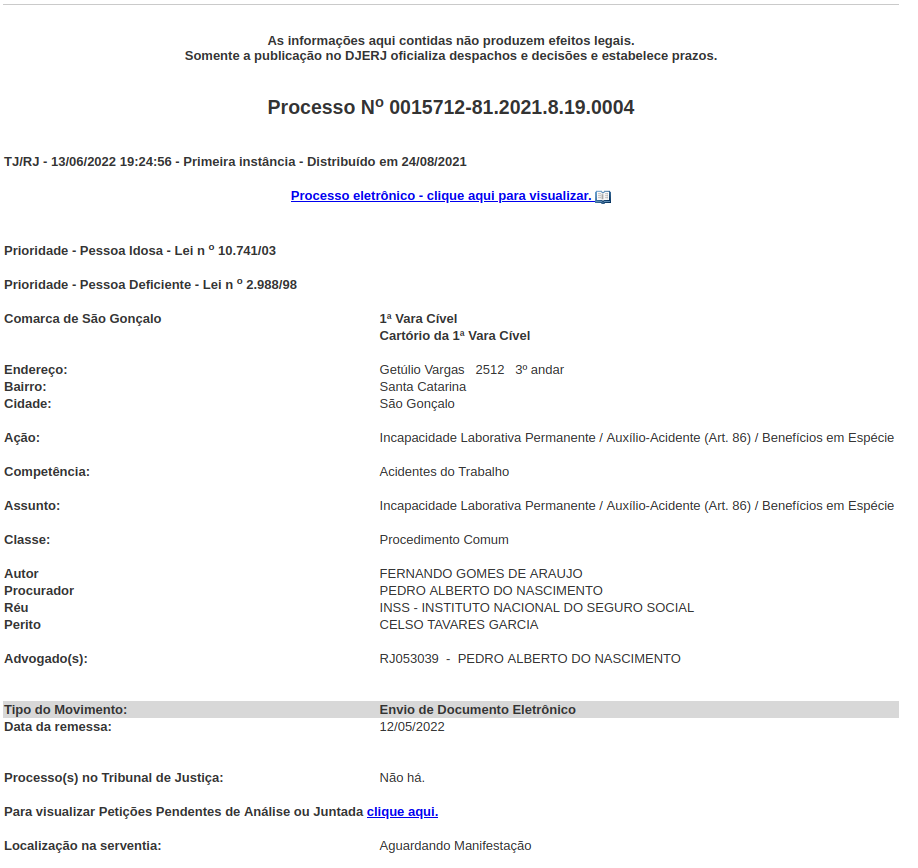
\includegraphics{img/exemplo-resultado-consulta-publica-1.png}
    \caption{%
        Página de resultado da consulta pública para o processo válido de
        número 2021.003.015548-9 (numeração
        antiga).\label{fig:exemplo-pagina-ww4}
    }
\end{figure}

\begin{listing}
    \centering{}
    \begin{minted}[autogobble,breaklines]{html}
        <tr>
          <td class="info" valign="top" nowrap="nowrap">Assunto:</td>
          <td valign="top">
            Incapacidade Laborativa Permanente / Auxílio-Acidente (Art. 86) / Benefícios em Espécie
          </td>
        </tr>
    \end{minted}
    \caption{Código HTML do campo ``Assunto:'' presente na~\Cref{fig:exemplo-pagina-ww4}.\label{cod:html-assunto}}
\end{listing}

A extração da informação de um campo é dada então \todo{:shrug:}

\begin{listing}[htb]
    \centering{}
    \begin{minted}[breaklines]{python}
        def extract_field(response: Response, field_text: str) -> str:
            field_xpath = f"//td[text()='{field_text}:']/following-sibling::td/text()"
            content = response.xpath(field_xpath).get().strip()
            return content
    \end{minted}
    \caption{%
        Código da função responsável pela extração de um campo em uma resposta
        de uma requisição a uma página de visualização de processo.
    }
    \label{cod:extract_field}
\end{listing}

\subsection{Estratégia alternativa: varredura com API JSON}

\begin{todolist}
    \item Iniciar descrevendo a relação entre parâmetros de busca da busca HTML
          e as rotas como \texttt{/por-numero/}.
    \item Expor sobre a existência de múltiplos sub-domínios do TJ-RJ;
    \item Complementar com a falta de documentação da API do TJ-RJ (forma de
          operação descoberta na base de tentativa e erro);
    \item Explicar rapidamente sobre a filtragem dos campos;
\end{todolist}

\section{Estratégias de aceleração de consulta}

\todo{%
    Para cada estratégia, nomeá-la para referenciar na parte de resultados
    demonstrando os ganhos de aceleração. Nesta seção, não tomar conclusões
    sobre ganhos, apenas enunciar e explicar como as estratégias funcionam e
    por que elas foram decididas dessa forma.
}

\todo{%
    Na seção de resultados, comparar um cenário base (sem aplicar as estratégias) com:
}
\begin{todolist}
    \item Apenas uma das estratégias aplicadas (fazer para cada estratégia);
    \item Com todas as estratégias aplicadas.
\end{todolist}
\todo{%
    A hipótese lançada é de que o maior tempo desprendido é com IO (e não
    processamento das requisições).
    A conclusão deverá confirmar essa hipótese demonstrando que com a redução
    (através de caching e através de requisições assíncronas) do gasto com IO o
    tempo de consulta se reduz de forma diretamente proporcional.
}

\subsection{Requisições assíncronas}

\subsection{\textit{Cache} dos resultados}

\begin{todolist}
    \item Justificar a necessidade de \textit{cache} para os resultados: em
          resumo, requisições, sejam de um mesmo usuário ou de usuários
          diferentes, podem muito bem conter uma intersecção dos processos que
          serão buscados.
\end{todolist}
